\documentclass{book}
 
%Russian-specific packages
%--------------------------------------
\usepackage[T2A]{fontenc}
\usepackage[utf8]{inputenc}
\usepackage[russian]{babel}
\usepackage{amsmath}
\usepackage{amssymb}
%--------------------------------------
 
%Hyphenation rules
%--------------------------------------
\usepackage{hyphenat}
\hyphenation{ма-те-ма-ти-ка вос-ста-нав-ли-вать доп-пель-ган-гер}
%--------------------------------------
 
\usepackage{graphicx}
\begin{document}
 
%\tableofcontents

\chapter[Что такое не везёт: p-values]{Что такое не везёт и как это рассчитывать: p-values}

\section*{Cтатистическая значимость}

Словосочетание <<статистическая значимость>> (или его психологического доппельгангера, <<достоверность>>), наверное, слышали все. Медицина, генетика, опросы про зубную пасту и против зубной пасты - весь этот поток информации без статистики, и без сравнения гипотез (вот для чего нужна значимость) превращается в хаос гиганстких данных.

Слово <<статистика имеет несколько значений. К более техническому, важному для нас, мы вернёмся позже, а сейчас поговорим немного общенаучном. Статистика и теория вероятности - это связанные способы исследования закономерностей мира. Теория вероятностей предсказывает события, исходя из моделей, и так пытается понять то, что мы видим вокруг. Монетка, игральная кость, нормальное распределение - всё это модели случайных переменных, а исходы этих переменных - это те события, которые мы можем увидеть - орёл, четыре, лист длиной 4 сантиметра. Статистика же делает для теории вероятности черновую, обратную работу. Чтобы модель заработала, нужно знать её параметры, и статистика и занимается тем, что по многим наблюдениям делает утверждения о параметрах модели. Иногда эти утверждения - это оценки параметров модели (мы много говорили об этом в предыдущей главе), а иногда - и мы сейчас будем говорить об этом случае - это заключения о пригодности модели для описания наблюдений.

\begin{figure}
    \centering
    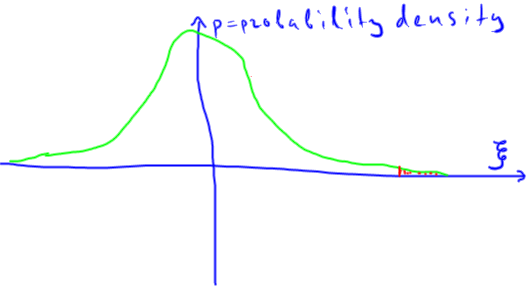
\includegraphics[scale=.5]{img/p-value.png}
    \caption{Площадь красного сегмента графика плотности вероятности случайной величины $\xi$ - это p-value, соответствующее значинию $\xi$ на границе сегмента}
    \label{pval}
\end{figure}



 
\end{document}
